In this chapter we will evaluate the architectures described in chapter \ref{chapter:architectures} with the method described in chapter \ref{chapter:design_of_experiments}. Some of them will additionally be evaluated with the implementation from chapter \ref{chapter:implementation}.







\section{Bandwidth}
When evaluating we are making some assumptions about bandwidth. Table \ref{tab:Bandwidth_latency} shows latency and bandwidth for different technologies. The WiFi bandwidths are based on data from CenturyLink\cite{noauthor_24_nodate}. The 4G and 5G bandwidths are real-world examples from 4g.co.uk\cite{noauthor_how_nodate}. The 4G latency are from ping tests, while the 5G latency are from Verizon\cite{noauthor_what_2020}.

\begin{table}[h!]
    \centering
    \begin{tabular}[c]{|c|c|c|}
        \hline
        Technology & Latency (ms) & Bandwidth (Mbps) \\
            &   &  Download/Upload \\
        \hline
        \hline
        Wifi (2.4GHz) & <=1 & 150/150  \\
        \hline
        Wifi (5GHz) & <=1 & 450/450  \\
        \hline
        4G & 30-65 & 42/25  \\
        \hline
        5G & 30 & 200/100  \\
        \hline
        Wired LAN & <=1 & 1000+  \\
        \hline
        WAN & 10-300+ & 1000+  \\
        \hline
        
        
    \end{tabular}
    \caption{Latency and bandwidth for different technologies.}
    \label{tab:Bandwidth_latency}
\end{table}
When doing calculations in this chapter, we will be using numbers from table \ref{tab:Bandwidth_latency}.









\section{Multi-Access Edge Computing} \label{section:MEC_evaluation}
MEC seeks to offload a reasonable amount of work. Therefore, we will not necessarily offload all the work, but rather test with several ratios of computation offloading. It is not always efficient to offload all the work. According to Mach and Becvar´s survey\cite{mach_mobile_2017}, we can divide offloading into three categories:
\begin{itemize}
    \item \textit{Local execution}, where all the work is done on the mobile device.
    \item \textit{Full offloading}, where we offload all work to server(s).
    \item \textit{Partial offloading}, where we offload some of the work, and do some local.
\end{itemize}
We will compare these three. We will also test different variations of Partial offloading. According to cpubenchmark\cite{noauthor_passmark_nodate}, flagship phones is about half as fast as a standard desktop CPU. We assume that we are dealing with below average CPU's cellphones, as most people do not have the flagship phone. We will test different strengths of the MEC Server. We assume that the data centre will have plenty of resources. In total, we want to do 10000 iterations spread over all the nodes.

\subsection{Local execution}
%lacking geographic location?
\begin{table}[h!]
    \centering
    \begin{tabular}[c]{|c|c|c|c|}
        \hline
        Node type & Limitation & Iterations & Time used (s) \\
        \hline
        \hline
        Local & 30 & 10000 & 333.6 \\
        \hline
    \end{tabular}
    \caption{Only local execution.}
    \label{tab:MEC_local_execution}
\end{table}
Table \ref{tab:MEC_local_execution} shows the time used for local execution only. This to show how long it would take if we do not use offloading.



\subsection{Full offloading}
%spread out over more nodes
\begin{table}[h!]
    \centering
    \begin{tabular}[c]{|c|c|c|c|}
        \hline
        Node type & Limitation & Iterations & Time used (s)\\
        \hline
        \hline
        Local & 30 & 0 & 0 \\
        \hline
        Near & 100 & 2500 & 23.3 \\
        \hline
        Far & 300 & 7500 & 30.5 \\
        \hline
    \end{tabular}
    \caption{Full offloading.}
    \label{tab:MEC_full_offloading}
\end{table}

\begin{table}[h!]
    \centering
    \begin{tabular}[c]{|c|c|c|c|}
        \hline
        Node type & Limitation & Iterations & Time used (s)\\
        \hline
        \hline
        Local & 30 & 0 & 0 \\
        \hline
        Near & 100 & 2800 & 27.3 \\
        \hline
        Far & 300 & 7200 & 29.8 \\
        \hline
    \end{tabular}
    \caption{Full offloading with more balance.}
    \label{tab:MEC_full_offloading_balanced}
\end{table}

Table \ref{tab:MEC_full_offloading} and \ref{tab:MEC_full_offloading_balanced} shows time used when offloading work to nodes that have little to no latency from Local (less than 1 ms). This essentially shows how much time is used on calculation if we have no communication between nodes.  

\begin{table}[h!]
    \centering
    \begin{tabular}[c]{|c|c|c|c|c|}
        \hline
        Node type & Limitation & Iterations & RTT to Local (ms)& Time used (s)\\
        \hline
        \hline
        Local & 30 & 0 & 0 & 0 \\
        \hline
        Near & 100 & 2800 & 30 & 92.8 \\
        \hline
        Far & 300 & 7200 & 170 & 1304.8 \\
        \hline
    \end{tabular}
    \caption{Full offloading with communication between Local and Near/Far.}
    \label{tab:MEC_full_offloading_latency}
\end{table}

Table \ref{tab:MEC_full_offloading_latency} shows how latency affects the work. Here, it will have to get data from Local after every iterations. There is a lot of communication between the nodes.

\begin{table}[h!]
    \centering
    \begin{tabular}[c]{|c|c|c|c|c|}
        \hline
        Node type & Limitation & Iterations & RTT to Local (ms)& Time used (s)\\
        \hline
        \hline
        Local & 30 & 0 & 0 & 0 \\
        \hline
        Near & 100 & 8500 & 30 & 279.3 \\
        \hline
        Far & 300 & 1500 & 170 & 267.9 \\
        \hline
    \end{tabular}
    \caption{Full offloading with communication and more balance in the nodes.}
    \label{tab:MEC_full_offloading_latency_balance}
\end{table}

Table \ref{tab:MEC_full_offloading_latency_balance} shows a more balanced workload distribution. The Near node is doing significantly more work. Here we also have to get data from Local after each iteration.














\subsection{Partial offloading}
For partial offloading, we want all nodes to work.
\begin{table}[h!]
    \centering
    \begin{tabular}[c]{|c|c|c|c|}
        \hline
        Node type & Limitation & Iterations & Time used (s)\\
        \hline
        \hline
        Local & 30 & 1000 & 33.0 \\
        \hline
        Near & 100 & 2000 & 19.5 \\
        \hline
        Far & 300 & 7000 & 30.6 \\
        \hline
    \end{tabular}
    \caption{Partial offloading.}
    \label{tab:MEC_partial_offloading}
\end{table}


\begin{table}[h!]
    \centering
    \begin{tabular}[c]{|c|c|c|c|}
        \hline
        Node type & Limitation & Iterations & Time used (s)\\
        \hline
        \hline
        Local & 30 & 850 & 28.1 \\
        \hline
        Near & 100 & 2700 & 26.5 \\
        \hline
        Far & 300 & 6450 & 29.1 \\
        \hline
    \end{tabular}
    \caption{Partial offloading with more balance.}
    \label{tab:MEC_partial_offloading_balanced}
\end{table}
Table \ref{tab:MEC_partial_offloading} and \ref{tab:MEC_partial_offloading_balanced} shows the result of offloading with less than 1 ms latency and little overhead.






\begin{table}[h!]
    \centering
    \begin{tabular}[c]{|c|c|c|c|c|}
        \hline
        Node type & Limitation & Iterations & RTT to Local (ms)& Time used (s)\\
        \hline
        \hline
        Local & 30 & 850 & 0 & 28.1 \\
        \hline
        Near & 100 & 2700 & 30 & 86.0 \\
        \hline
        Far & 300 & 6450 & 170 & 1131.2 \\
        \hline
    \end{tabular}
    \caption{Partial offloading with communication between Local and Near/Far.}
    \label{tab:MEC_partial_offloading_latency}
\end{table}

Table \ref{tab:MEC_partial_offloading_latency} shows how latency affects offloading. We have the same configuration as shown in table \ref{tab:MEC_partial_offloading_balanced}, but now the nodes are spread out and have latency affecting the offloading. The nodes have to get data from Local after each iteration.

\begin{table}[h!]
    \centering
    \begin{tabular}[c]{|c|c|c|c|c|}
        \hline
        Node type & Limitation & Iterations & RTT to Local (ms)& Time used (s)\\
        \hline
        \hline
        Local & 30 & 4550 & 0 & 151.3  \\
        \hline
        Near & 100 & 4525 & 30 & 149.8 \\
        \hline
        Far & 300 & 925 & 170 & 163.0 \\
        \hline
    \end{tabular}
    \caption{Partial offloading with communication and more balance in the nodes.}
    \label{tab:MEC_partial_offloading_latency_balance}
\end{table}


Table \ref{tab:MEC_full_offloading_latency_balance} shows a more balanced version. We can see that more of the work happens locally and on the node with less latency.

\subsection{Decreasing interaction}

\begin{figure}[t]
    \centering
    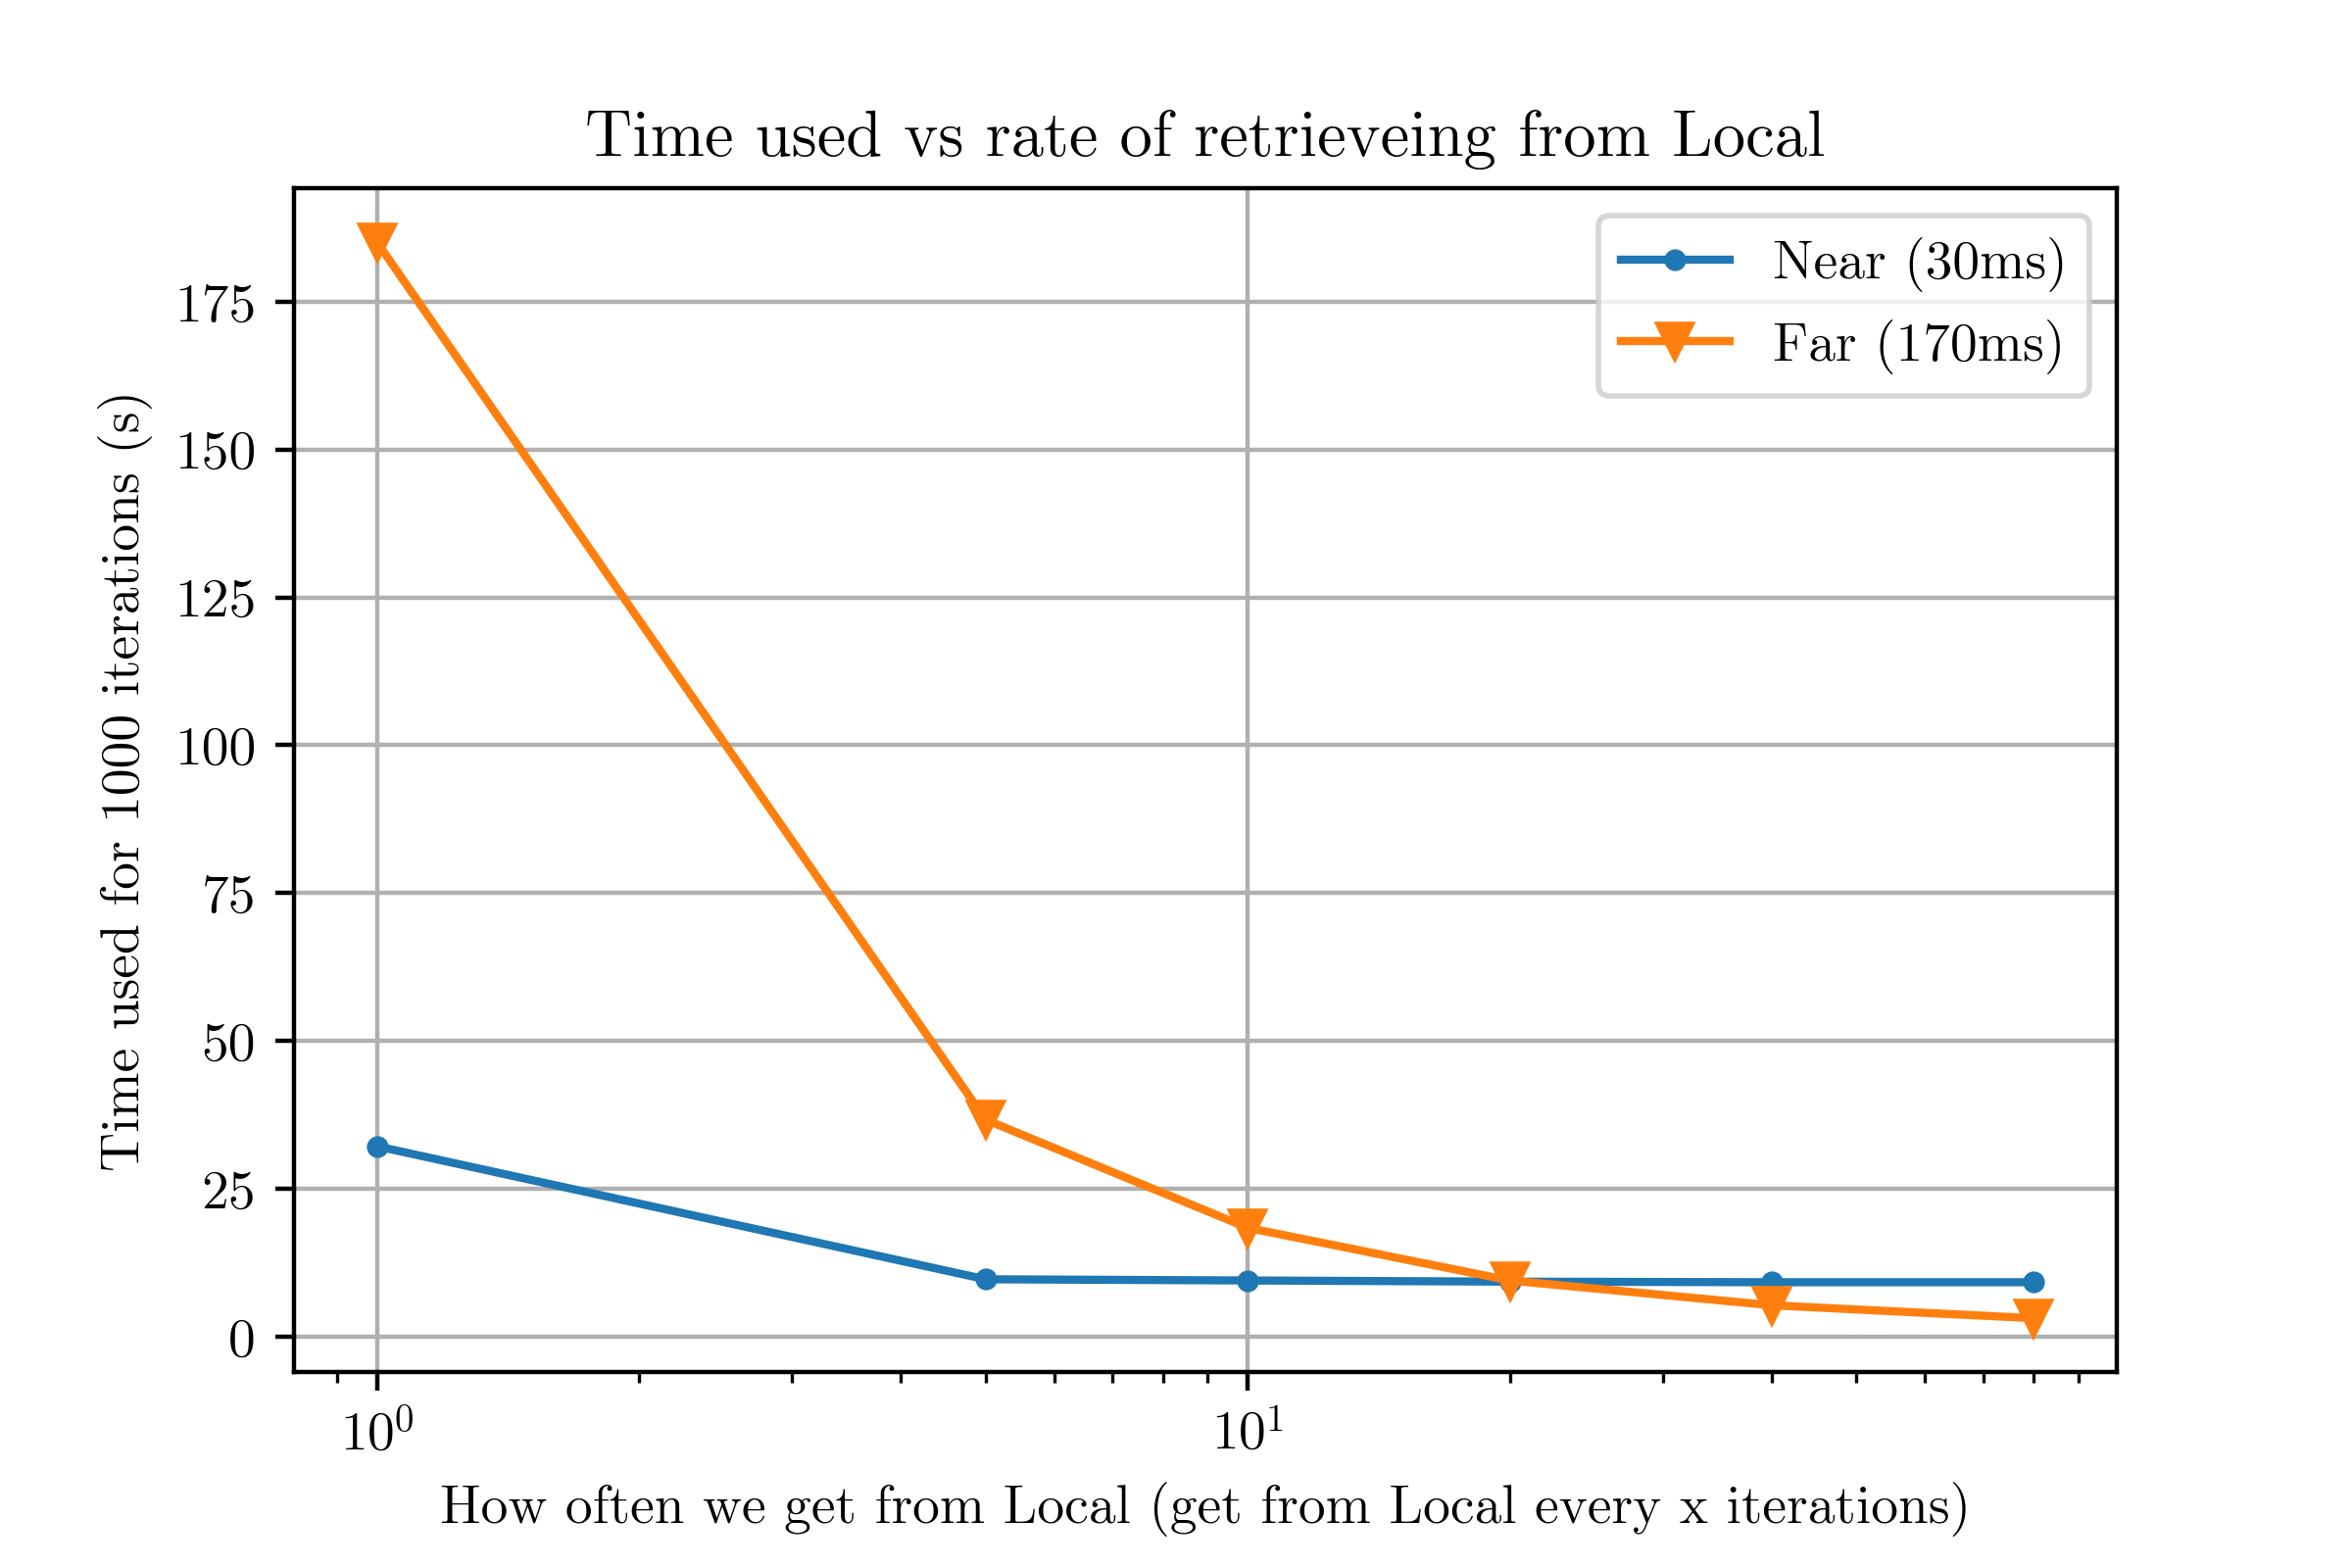
\includegraphics[scale=1]{chapters/evaluation/figures/times.png}
    \caption{Graph showing how interaction hurts. If x=10 then we get from Local every 10 iterations.}
    \label{fig:time_graph_near_far}
\end{figure}

Figure \ref{fig:time_graph_near_far} shows how latency affects the time used when you have to constantly get data from the Local device. We have tested with various frequencies of interaction. The graph essentially shows how much time is used on Near or Far node with regards to how often it has to get data from the Local node. 
\begin{figure}[t]
    \centering
    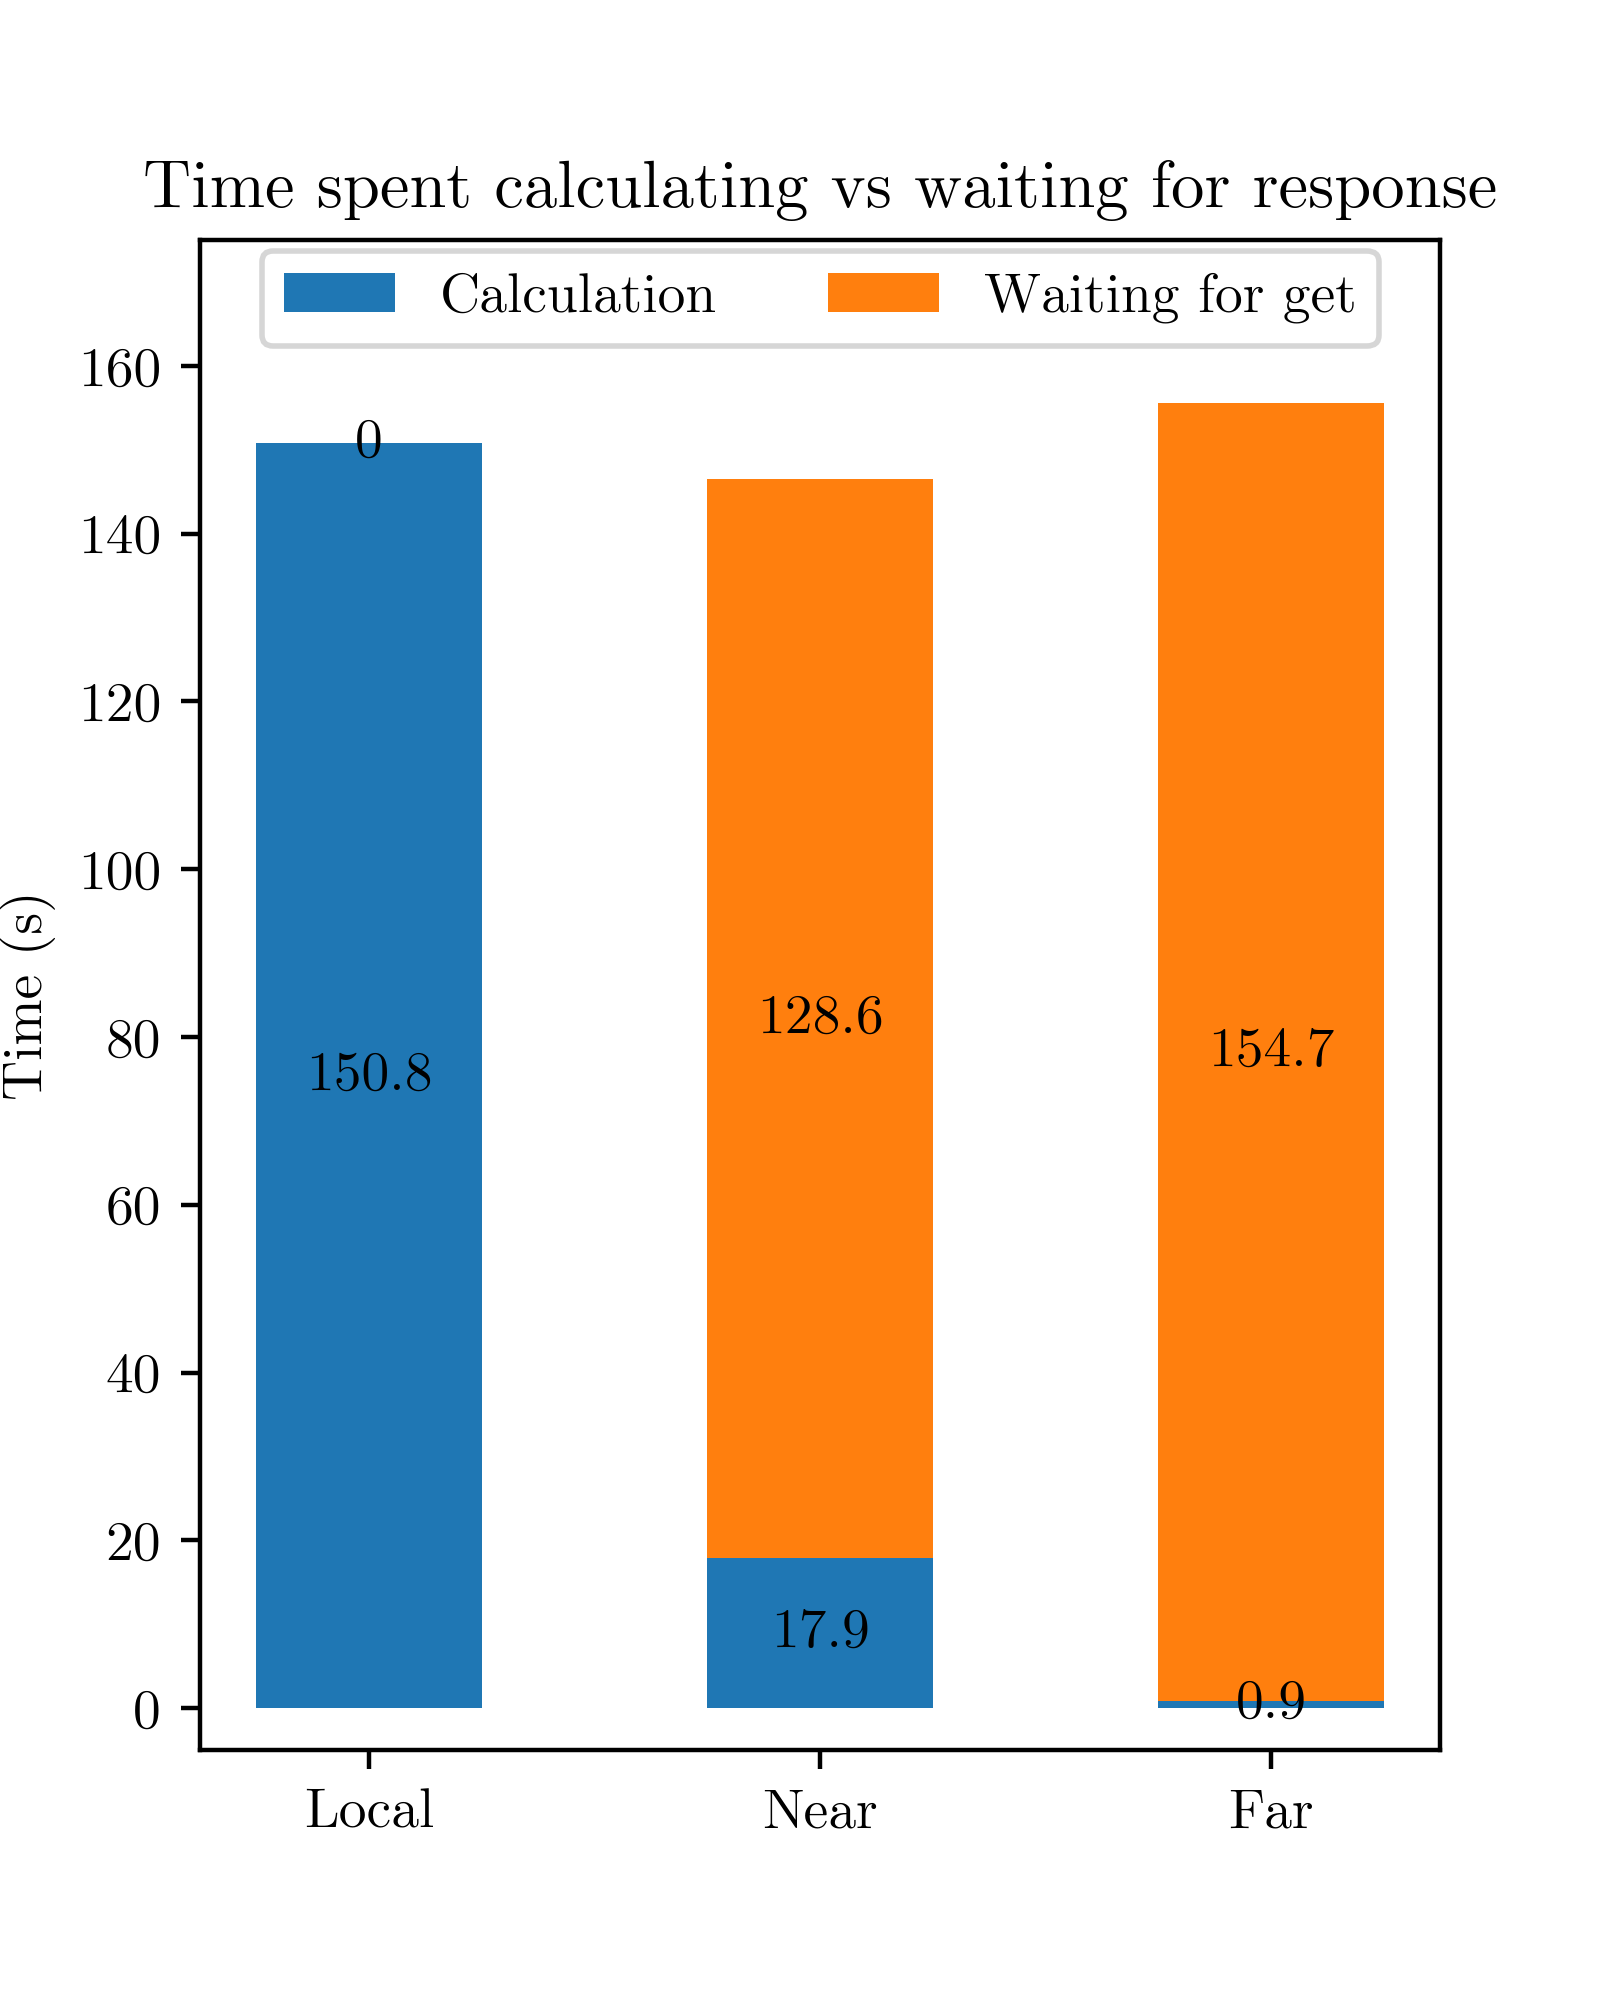
\includegraphics[scale=1]{chapters/evaluation/figures/bar_local_near_far_compare.png}
    \caption{Illustration of how much time is spent on waiting for data due to latency when using MEC Server.}
    \label{fig:bar_local_near_far}
\end{figure}

Figure \ref{fig:bar_local_near_far} shows how latency affect the the total time used when we have to constantly get data from the local device. It uses the same configuration as shown in table \ref{tab:MEC_partial_offloading_latency_balance}.




\subsection{Comparison of results} \label{subsection:MEC_comparison}%Discussion of mec?
By comparing table \ref{tab:MEC_full_offloading_latency_balance} and \ref{tab:MEC_partial_offloading_latency_balance} we can see that we get faster results by using Partial offloading. Because the nodes work in parallel, the node who used the longest time shows how much time were used from start to end. Therefore, Partial offloading is the best solution for having fastest result when there is a lot of interaction.


Full offloading might for some devices be a requirement. The two most likely causes for this is if the Local device have very limited computational power, or need to save battery. Computation offloading is a great strategy to save energy, as sending data is usually not as expensive as computation. However, if we compare table \ref{tab:MEC_full_offloading_latency_balance} and \ref{tab:MEC_partial_offloading_latency_balance}, we can clearly see that using the local device will give results faster.

Table \ref{fig:bar_local_near_far} shows that if the Near and Far node constantly have to get data from Local, the time to complete the whole task will be much slower. If you don't need to get info that often, then the Far server will yield better results as it has more computational power. In other words, the more interaction the better it is to use Local or Near node more. When there is little interaction then it is best to use the Far node more.


%nevn offloading. Vis stolpediagramm hvor en chunk av tiden er offloading. Vis også med N*latency?
%Bar chart med som viser hvor stor andel av de forskjellige utregningene som består av calulation og latency






\subsection{Characteristics}
\subsubsection{Control}
As discussed in section \ref{section:MEC_architecture}, the architecture of MEC is up to the programmers. They can use NFV and SDN to control how each mobile device will be able to use the architecture. They can in other words use SDN and NFV to tailor the network to the context.
\subsubsection{Offloading}
Since they use the cellular network to offload work, this architecture is well suited for IoT devices that can afford the latency. The cellular network is ubiquitous in modern society, and therefore it is optimal for IoT devices that move a lot, e.g. self-driving cars. When offloading they have to upload something, e.g. a VM, to the MEC Server. Alternatively they can make the MEC Server download from elsewhere.
\subsubsection{Distribution}
MEC is easily horizontally scalable, as more MEC Servers can easily be added to cell towers. The only limit is how much power there is available and how much space there is available. If only a few servers is needed, then the cost is not too high either. It is also easily scalable in the sense that you can add more VMs to the MEC Server to help with offloading if needed. 
\subsubsection{Security?}
TODO

%offloading
%    compute 
%    storage
%distribution
%    scaling
%Control


%tabell? subsections? idk

%TODO
% Gjøre målinger med overføring av filer først. Finn data på bandwidth og pluss det på tiden.
% Gjøre målinger hvor det kreves mer samhandling mellom nodene. Vi må se latency!


%\cite{mach_mobile_2017} for hvor mye som skal offloades.!!!!
% test med 100% offload, 50% offload osv
%\begin{itemize}
 %   \item Easily scalable as we have the common interface. This makes it easy to add more vms to run more apps. So, its horizontally scalable?
%\end{itemize}







\section{Cloudlets}
For Cloudlets we will also test with Full and Partial offloading like in section \ref{section:MEC_evaluation}. The same metrics for limitations for each type of node is also used. In total we want to do 10000 iterations spread over all the nodes.

\subsection{Full execution}
\begin{table}[h!]
    \centering
    \begin{tabular}[c]{|c|c|c|c|c|}
        \hline
        Node type & Limitation & Iterations & RTT to Local (ms)& Time used (s)\\
        \hline
        \hline
        Local           & 30 & 0 & 0 & 0  \\
        \hline
        Cloudlet(Near)  & 100 & 2800 & 3 & 30.2 \\
        \hline
        Far             & 300 & 7200 & 170 & 1285.0 \\
        \hline
    \end{tabular}
    \caption{Full offloading with communication.}
    \label{tab:Cloudlet_full_offloading_latency}
\end{table}
Table \ref{tab:Cloudlet_full_offloading_latency} shows the result of Full offloading to a nearby Cloudlet. We have used the same configuration as in table \ref{tab:MEC_full_offloading_balanced} to show how latency affects the result. 

\begin{table}[h!]
    \centering
    \begin{tabular}[c]{|c|c|c|c|c|}
        \hline
        Node type & Limitation & Iterations & RTT to Local (ms)& Time used (s)\\
        \hline
        \hline
        Local           & 30 & 0 & 0 & 0  \\
        \hline
        Cloudlet(Near)  & 100 & 9500 & 3 & 98.8 \\
        \hline
        Far             & 300 & 500 & 170 & 94.6 \\
        \hline
    \end{tabular}
    \caption{Full offloading with communication with more balance.}
    \label{tab:Cloudlet_full_offloading_latency_balanced}
\end{table}
Table \ref{tab:Cloudlet_full_offloading_latency_balanced} shows the result of a more balanced configuration with Full offloading in the sense that they used about the same time.




\subsection{Partial offloading}
\begin{table}[h!]
    \centering
    \begin{tabular}[c]{|c|c|c|c|c|}
        \hline
        Node type & Limitation & Iterations & RTT to Local (ms)& Time used (s)\\
        \hline
        \hline
        Local           & 30 & 850 & 0 & 28.1  \\
        \hline
        Cloudlet(Near)  & 100 & 2700 & 3 & 27.8 \\
        \hline
        Far             & 300 & 6450 & 170 & 1188.4 \\
        \hline
    \end{tabular}
    \caption{Partial offloading with communication.}
    \label{tab:Cloudlet_partial_offloading_latency}
\end{table}
Table \ref{tab:Cloudlet_partial_offloading_latency} shows the result of Partial offloading to a nearby Cloudlet. We have used the same configuration as in table \ref{tab:MEC_partial_offloading_balanced} to show how latency affects the result. 





\begin{table}[h!]
    \centering
    \begin{tabular}[c]{|c|c|c|c|c|}
        \hline
        Node type & Limitation & Iterations & RTT to Local (ms)& Time used (s)\\
        \hline
        \hline
        Local           & 30 & 2400 & 0 & 79.2  \\
        \hline
        Cloudlet(Near)  & 100 & 7150 & 3 & 73.3 \\
        \hline
        Far             & 300 & 450 & 170 & 75.2 \\
        \hline
    \end{tabular}
    \caption{Partial offloading with communication with more balance.}
    \label{tab:Cloudlet_partial_offloading_latency_balanced}
\end{table}
Table \ref{tab:Cloudlet_partial_offloading_latency_balanced} shows the result of a more balanced configuration with Partial offloading in the sense that they used about the same time.







\subsection{Decreasing interaction}
\begin{figure}[t]
    \centering
    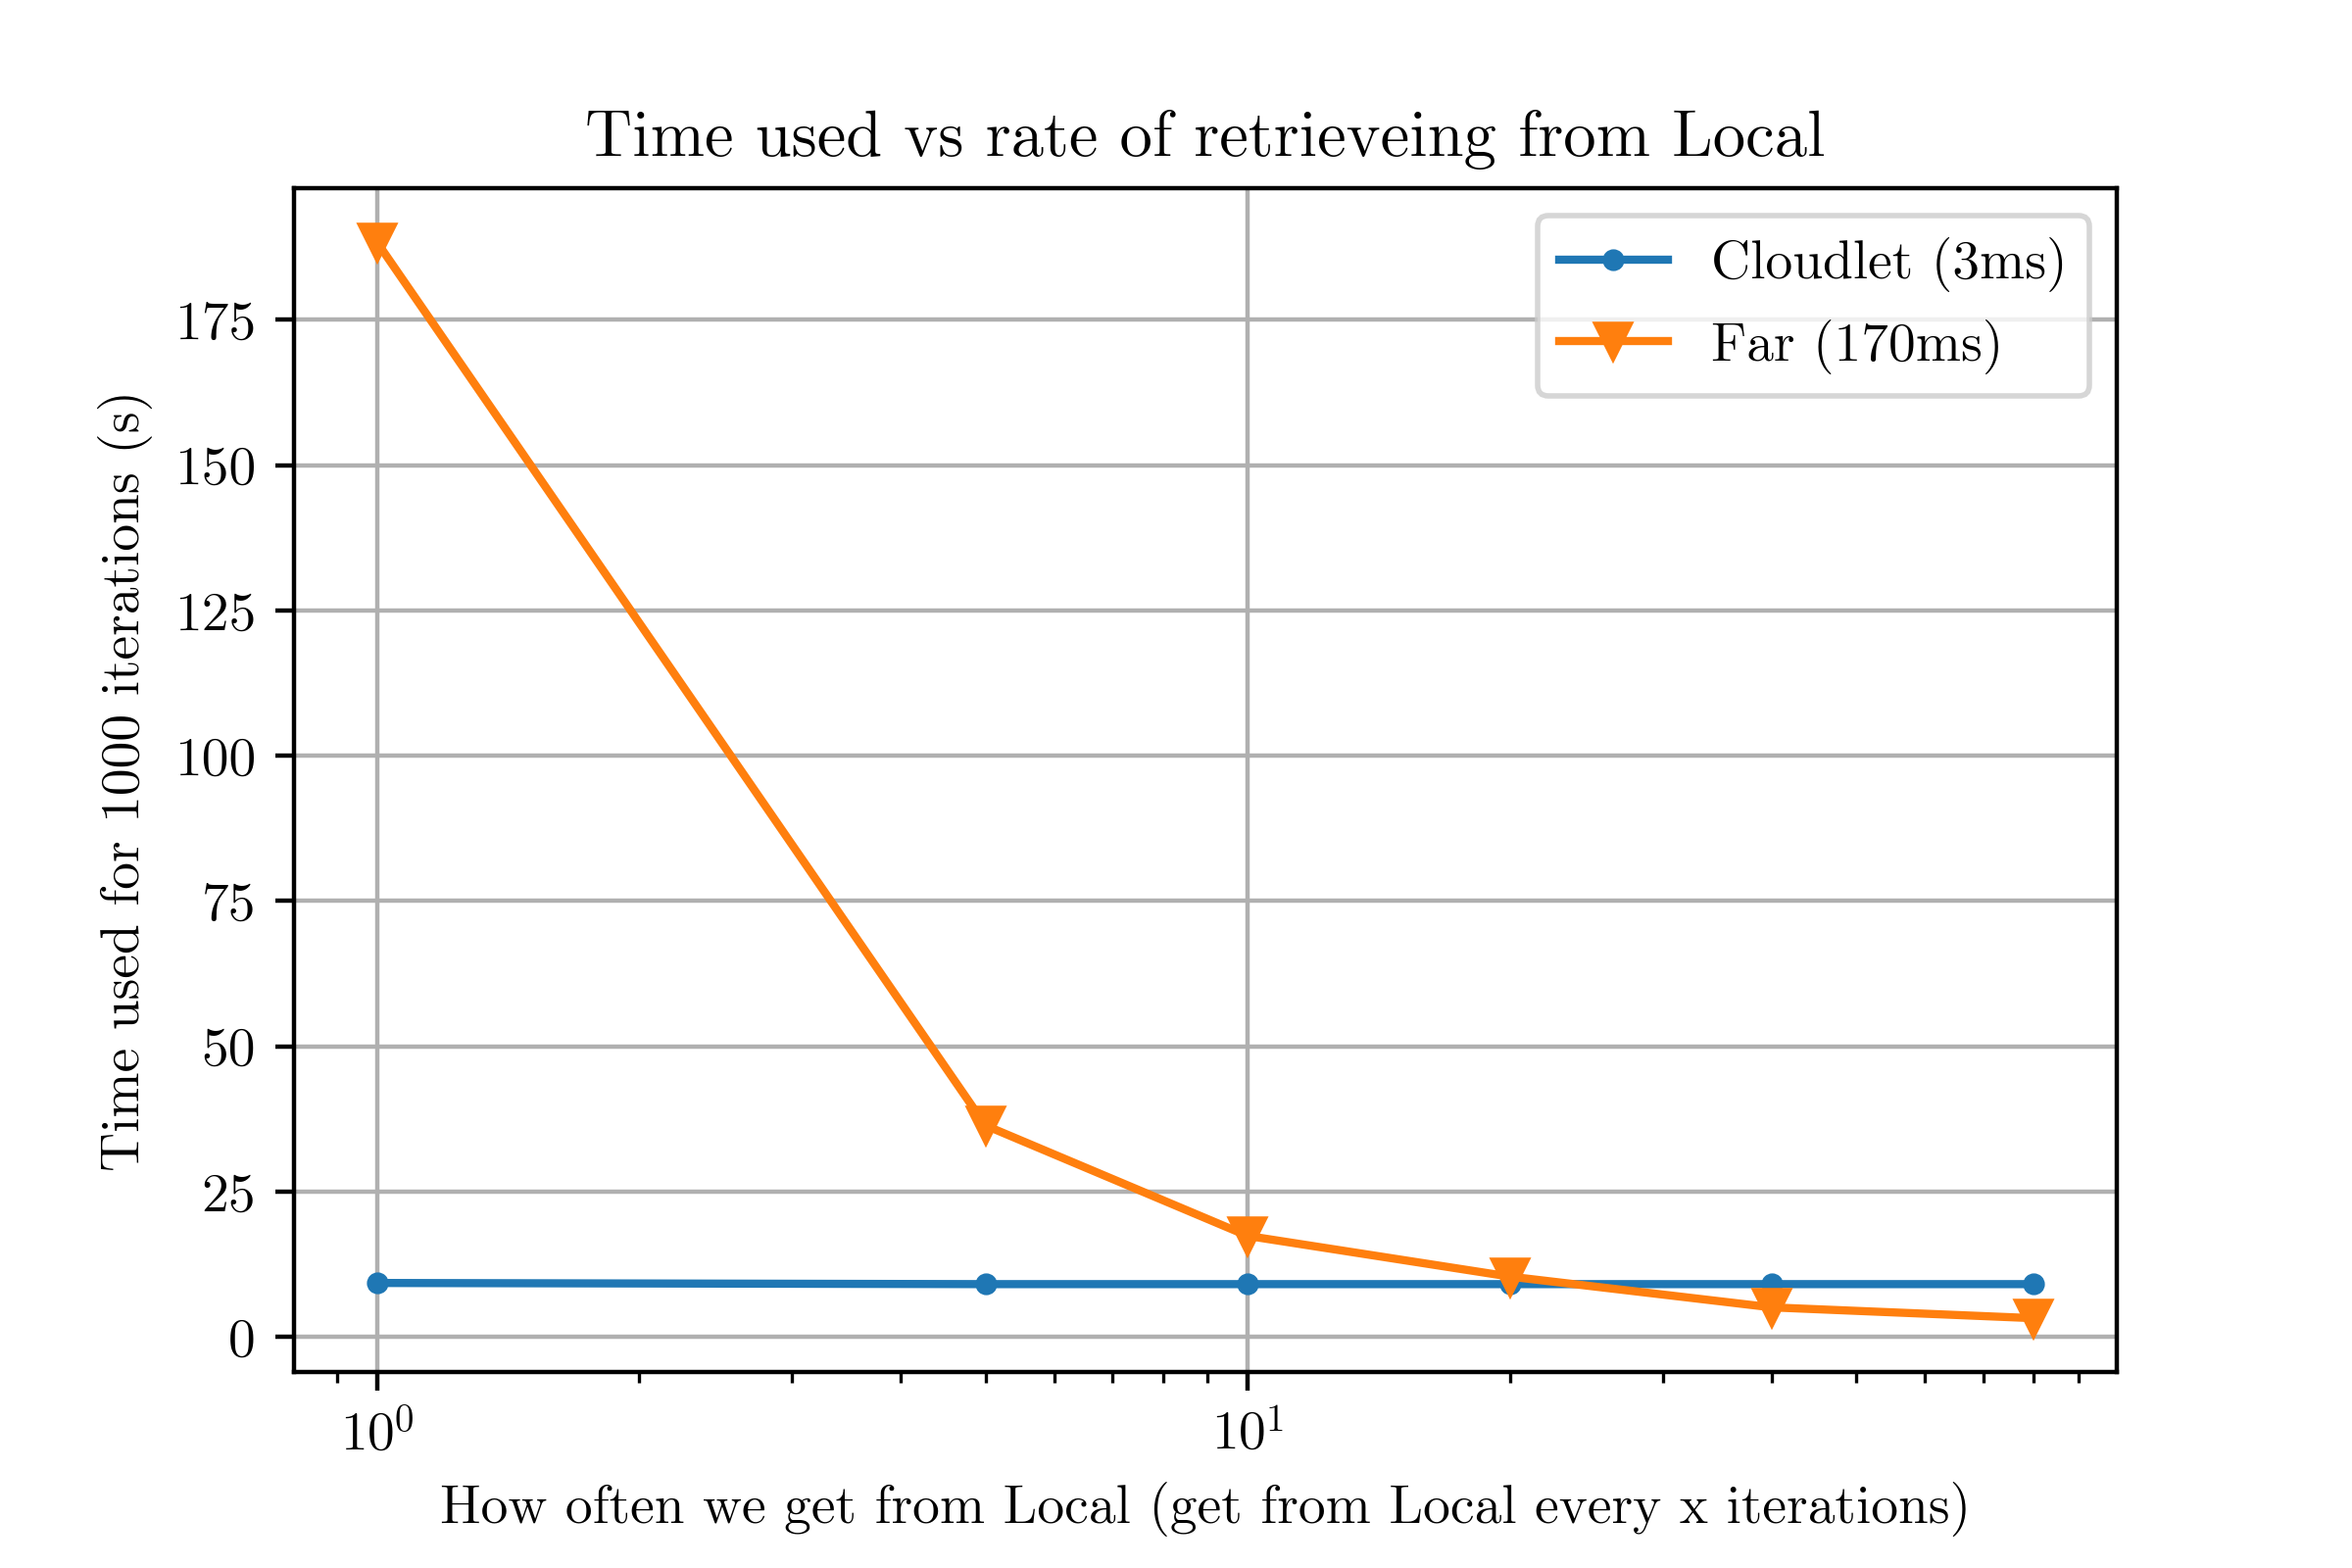
\includegraphics[scale=1]{chapters/evaluation/figures/Cloudlet_latency.png}
    \caption{Graph showing how interaction hurts. If x=10 then we get from Local every 10 iterations.}
    \label{fig:Cloudlet_latency_near_far_comparison}
\end{figure}
Figure \ref{fig:Cloudlet_latency_near_far_comparison} shows how the frequency of interaction between nodes will affect the time used, like shown for MEC in \ref{fig:time_graph_near_far}. 


\begin{figure}[t]
    \centering
    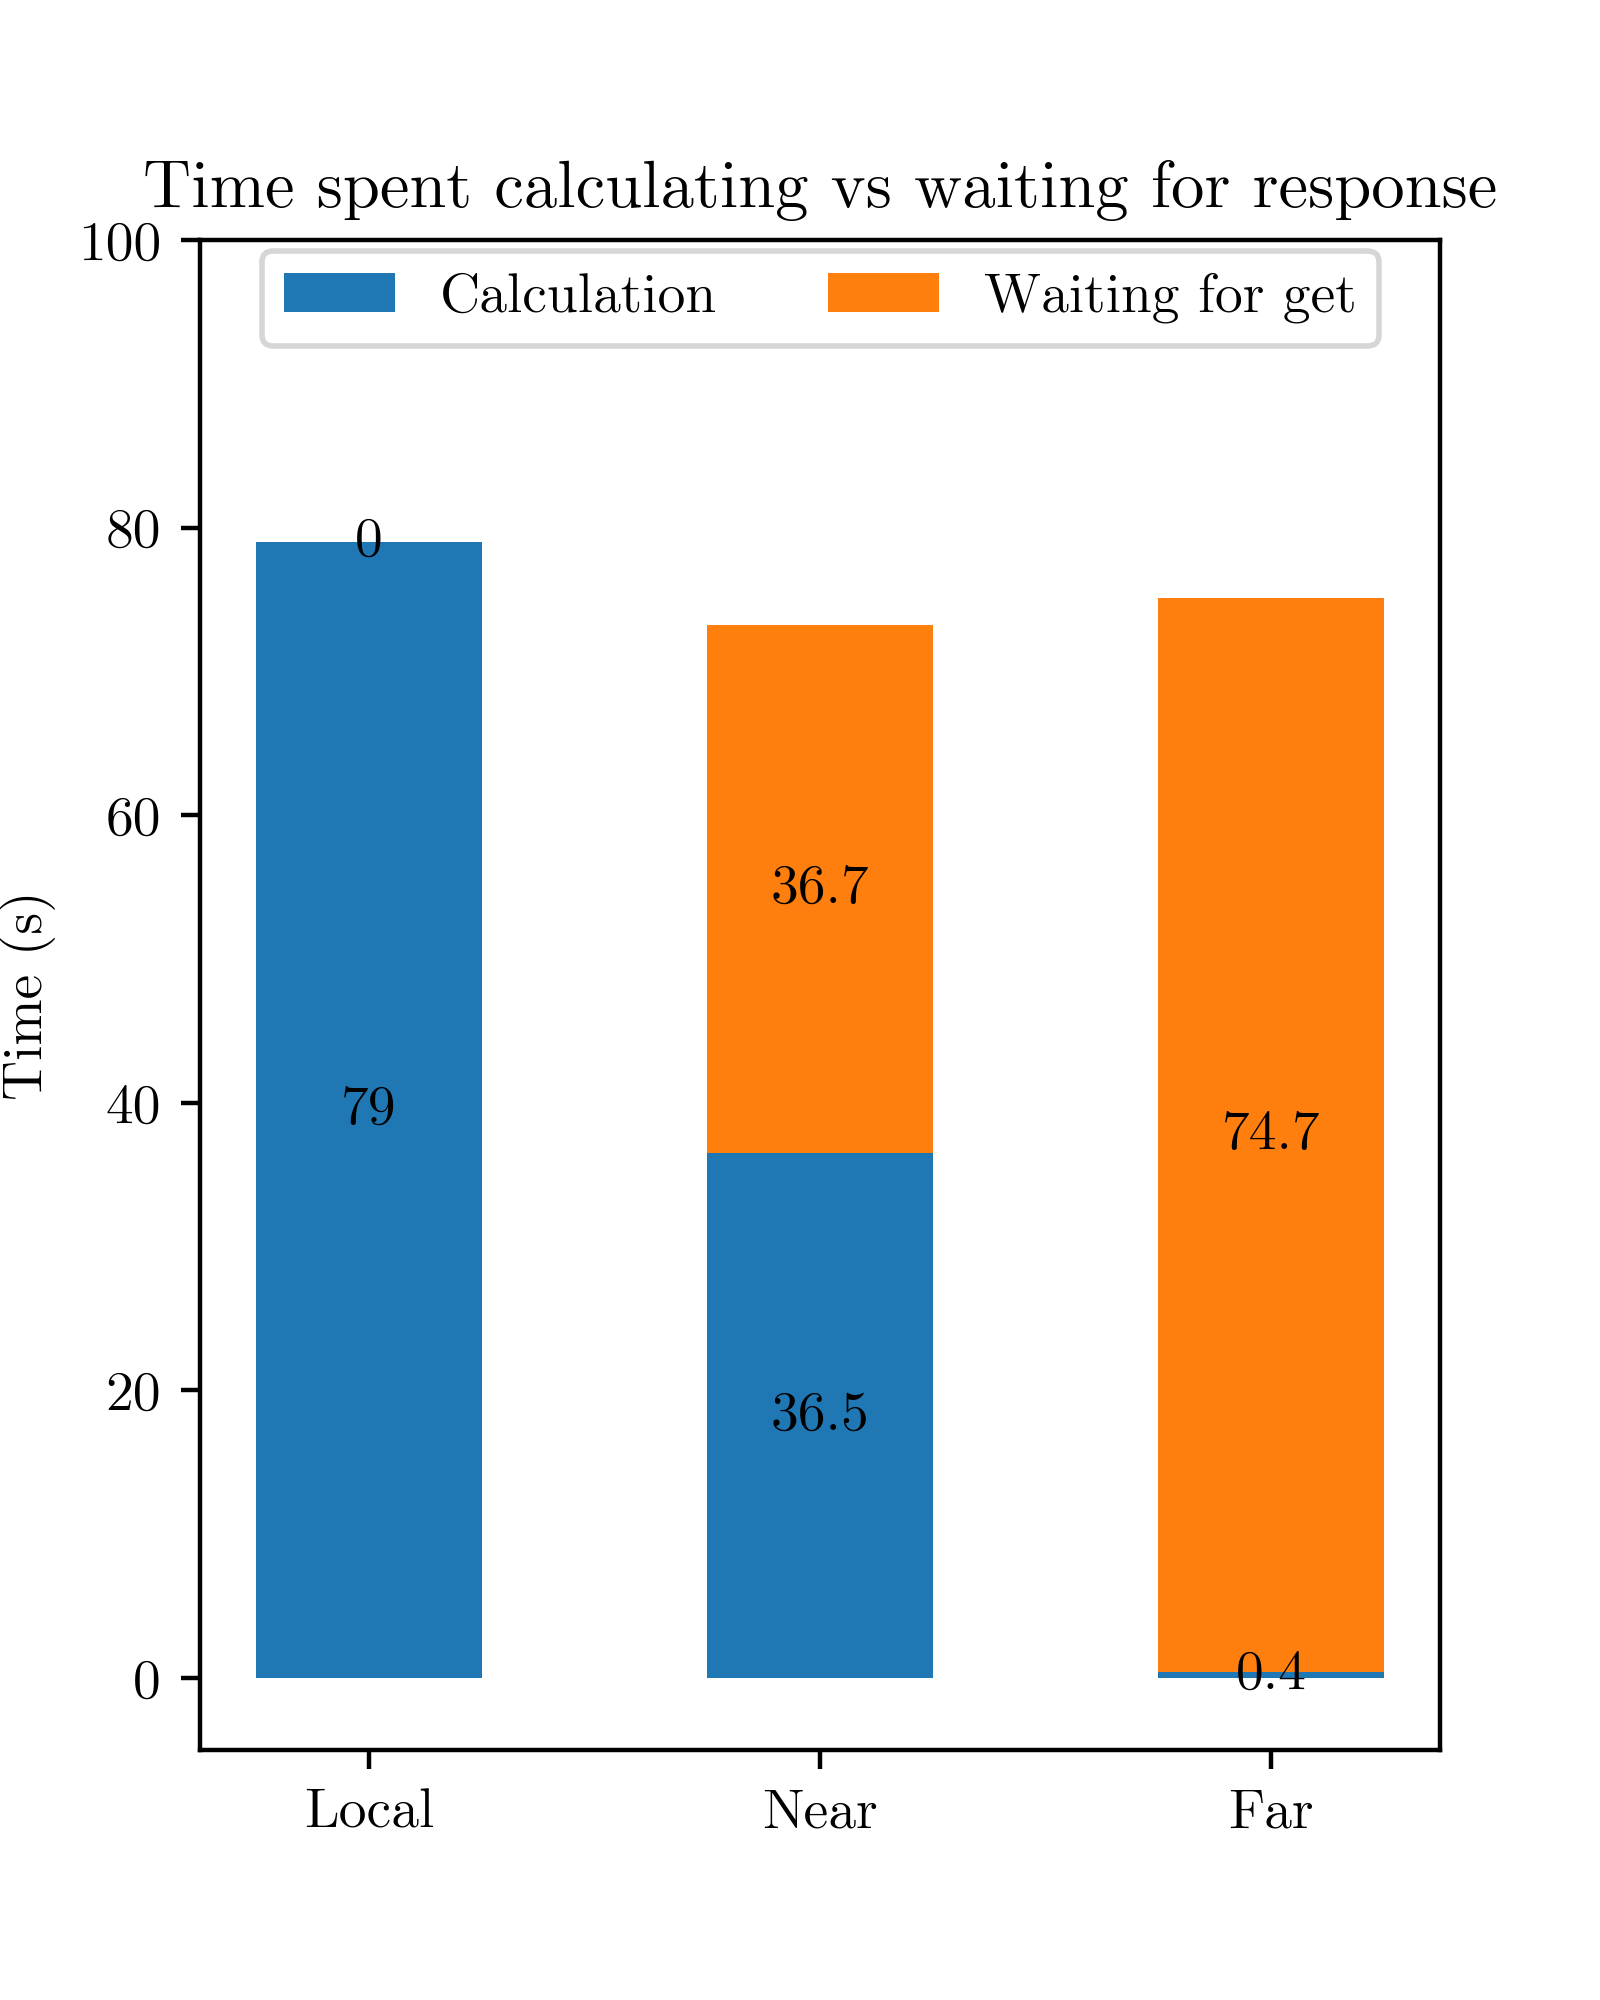
\includegraphics[scale=1]{chapters/evaluation/figures/Cloudlet_bar_latency.png}
    \caption{Illustration of how much time is spent on waiting for data due to latency when using Cloudlets.}
    \label{fig:Cloudlet_latency_bar}
\end{figure}
Figure \ref{fig:Cloudlet_latency_bar} shows how much time used on waiting for data from Local, compared to how much time is used on calculating. The configuration used here is the same as shown in table \ref{tab:Cloudlet_partial_offloading_latency_balanced}.




\subsection{Comparison of results}
By comparing table \ref{tab:Cloudlet_full_offloading_latency_balanced} and \ref{tab:Cloudlet_partial_offloading_latency_balanced} we can see that we benefit from also using the Local device. However, if the device that is using the Cloudlets require Full offloading, then we still have significant speedup by offloading to the Cloudlet and the Far node compared to Local execution.

Figure \ref{fig:Cloudlet_latency_near_far_comparison} shows that we can get better results by using Far in the situation where interaction between nodes is low. In other words, Cloudlets can benefit from using Far, but only when there is little communication needed. For fast response times we need to use the Cloudlet to do the computation. 

Figure \ref{fig:Cloudlet_latency_bar} shows that having the lower latency than MEC is beneficial. More time is used on calculation rather than waiting on data.



\subsection{Characteristics}
\subsubsection{Control}
Controlling Cloudlets is done by the owner of each Cloudlet. Since Cloudlets are to be placed on locations, e.g. a coffee shop, then the owner of that location is able to configure the Cloudlet. The location owner can then limit usage and limit what kinds of applications are used on the Cloudlet.
\subsubsection{Offloading}
Cloudlets use \textit{dynamic VM synthesis} \cite{satyanarayanan_case_2009} to offload work. Essentially it means that we have to give the Cloudlet a VM to run the application. This gives an overhead, which they reported to be quite high. However, this has likely been improved since 2009 as technology has improved. 
\subsubsection{Distribution}
Distribution is expensive for Cloudlets. Satyanarayanan et al.\cite{satyanarayanan_case_2009} purposes different payment models, but each owner of a location has to decide if it is worth the investment. Since they are supposed to be ubiquitous, the total cost of having these readily available everywhere in society will be significant. 
\subsubsection{Security?}
TODO

\section{Google Anthos}

\section{Amazon Cloudfront}
TODO: Warm up time for lambda.

\section{Akamai}


\section{Discussion of findings}
TODO
Therefore, a balance of offloading is needed to adapt to each context.
 
Comparing MEC and cloudlets, Cloudlets have to migrate their program. MEC might have to, but dont generally have the same problem, as Cellular will work for quite a large area.

Comparing the results of Cloudlets and MEC Servers, then we can see that having less latency like the Cloudlet is preferable for better results. Howver one could argue that installation of MEC Servers are significantly easier. (TODO because...)


MEC and Cloudlets both have migration overhead, while the others do not.

Sometimes the result of the far is not relevant for the near. We can also let the near compute while the far stores data.

Near-Far computing is applicable where there is not much need for interaction between the Far node and the Local or Near node.

\section{Summary}
TODO
